\documentclass{standalone}
\usepackage{tikz}
\usetikzlibrary{patterns, positioning}

\begin{document}
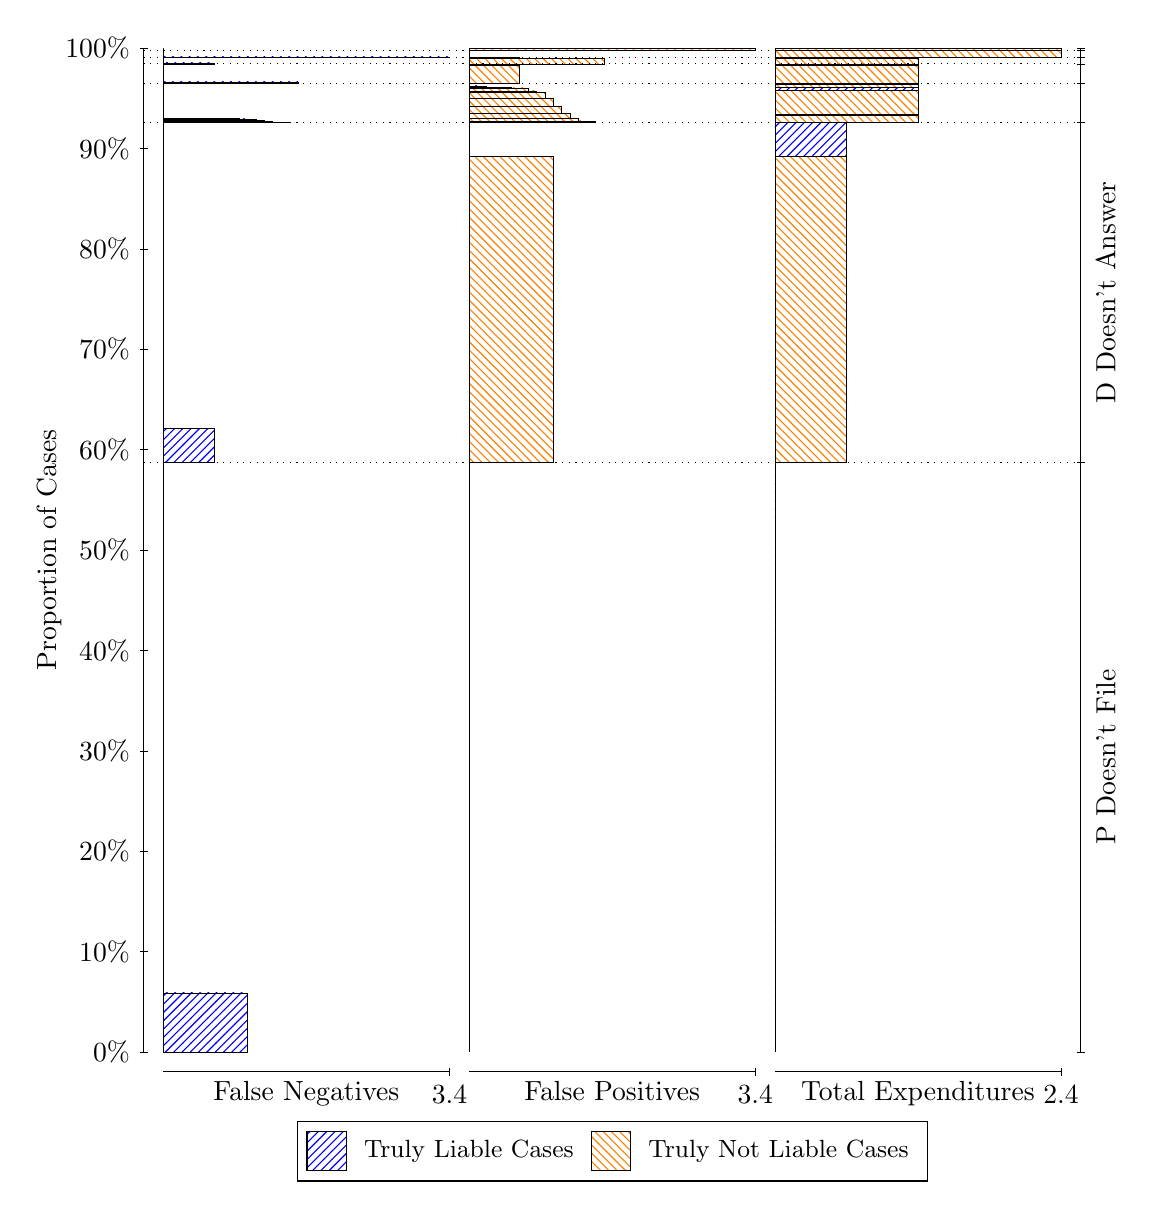
\begin{tikzpicture}
\draw[black, very thin] (1.5,1.75) -- (1.5,14.5);
\node[rotate=90, anchor=center] at (0.3, 8.125) {Proportion of Cases};
\draw[black, very thin] (1.45,1.75) -- (1.55,1.75);
\node[anchor=east] at (1.45, 1.75) {0\%};
\draw[black, very thin] (1.45,3.025) -- (1.55,3.025);
\node[anchor=east] at (1.45, 3.025) {10\%};
\draw[black, very thin] (1.45,4.3) -- (1.55,4.3);
\node[anchor=east] at (1.45, 4.3) {20\%};
\draw[black, very thin] (1.45,5.575) -- (1.55,5.575);
\node[anchor=east] at (1.45, 5.575) {30\%};
\draw[black, very thin] (1.45,6.85) -- (1.55,6.85);
\node[anchor=east] at (1.45, 6.85) {40\%};
\draw[black, very thin] (1.45,8.125) -- (1.55,8.125);
\node[anchor=east] at (1.45, 8.125) {50\%};
\draw[black, very thin] (1.45,9.4) -- (1.55,9.4);
\node[anchor=east] at (1.45, 9.4) {60\%};
\draw[black, very thin] (1.45,10.675) -- (1.55,10.675);
\node[anchor=east] at (1.45, 10.675) {70\%};
\draw[black, very thin] (1.45,11.95) -- (1.55,11.95);
\node[anchor=east] at (1.45, 11.95) {80\%};
\draw[black, very thin] (1.45,13.225) -- (1.55,13.225);
\node[anchor=east] at (1.45, 13.225) {90\%};
\draw[black, very thin] (1.45,14.5) -- (1.55,14.5);
\node[anchor=east] at (1.45, 14.5) {100\%};

\draw[black, very thin] (13.4,1.75) -- (13.4,14.5);
\draw[black, very thin] (13.35,1.75) -- (13.45,1.75);
\node[anchor=west] at (13.35, 1.75) {};
\draw[black, very thin] (13.35,9.2417) -- (13.45,9.2417);
\node[anchor=west] at (13.35, 9.2417) {};
\draw[black, very thin] (13.35,13.552) -- (13.45,13.552);
\node[anchor=west] at (13.35, 13.552) {};
\draw[black, very thin] (13.35,14.049) -- (13.45,14.049);
\node[anchor=west] at (13.35, 14.049) {};
\draw[black, very thin] (13.35,14.299) -- (13.45,14.299);
\node[anchor=west] at (13.35, 14.299) {};
\draw[black, very thin] (13.35,14.384) -- (13.45,14.384);
\node[anchor=west] at (13.35, 14.384) {};
\draw[black, very thin] (13.35,14.472) -- (13.45,14.472);
\node[anchor=west] at (13.35, 14.472) {};
\draw[black, very thin] (13.35,14.5) -- (13.45,14.5);
\node[anchor=west] at (13.35, 14.5) {};

\draw[black, very thin, pattern color=blue, pattern=north east lines] (1.75,1.75) rectangle (2.8186,2.4992);
\draw[black, very thin, pattern color=orange, pattern=north west lines] (1.75,2.4992) rectangle (1.75,9.2417);
\draw[black, very thin, pattern color=blue, pattern=north east lines] (1.75,9.2417) rectangle (2.3912,9.6708);
\draw[black, very thin, pattern color=orange, pattern=north west lines] (1.75,9.6708) rectangle (1.75,13.552);
\draw[black, very thin, pattern color=blue, pattern=north east lines] (1.75,13.552) rectangle (3.3529,13.556);
\draw[black, very thin, pattern color=blue, pattern=north east lines] (1.75,13.556) rectangle (3.2461,13.558);
\draw[black, very thin, pattern color=blue, pattern=north east lines] (1.75,13.558) rectangle (3.1392,13.567);
\draw[black, very thin, pattern color=blue, pattern=north east lines] (1.75,13.567) rectangle (3.0324,13.58);
\draw[black, very thin, pattern color=blue, pattern=north east lines] (1.75,13.58) rectangle (2.9255,13.593);
\draw[black, very thin, pattern color=blue, pattern=north east lines] (1.75,13.593) rectangle (2.8186,13.599);
\draw[black, very thin, pattern color=blue, pattern=north east lines] (1.75,13.599) rectangle (2.7118,13.603);
\draw[black, very thin, pattern color=blue, pattern=north east lines] (1.75,13.603) rectangle (2.6049,13.605);
\draw[black, very thin, pattern color=blue, pattern=north east lines] (1.75,13.605) rectangle (2.498,13.606);
\draw[black, very thin, pattern color=orange, pattern=north west lines] (1.75,13.606) rectangle (1.75,14.049);
\draw[black, very thin, pattern color=blue, pattern=north east lines] (1.75,14.049) rectangle (3.4598,14.069);
\draw[black, very thin, pattern color=orange, pattern=north west lines] (1.75,14.069) rectangle (1.75,14.299);
\draw[black, very thin, pattern color=blue, pattern=north east lines] (1.75,14.299) rectangle (2.3912,14.31);
\draw[black, very thin, pattern color=orange, pattern=north west lines] (1.75,14.31) rectangle (1.75,14.384);
\draw[black, very thin, pattern color=blue, pattern=north east lines] (1.75,14.384) rectangle (5.3833,14.387);
\draw[black, very thin, pattern color=orange, pattern=north west lines] (1.75,14.387) rectangle (1.75,14.472);
\draw[black, very thin, pattern color=orange, pattern=north west lines] (1.75,14.472) rectangle (1.75,14.491);
\draw[black, very thin, pattern color=blue, pattern=north east lines] (1.75,14.491) rectangle (1.75,14.5);
\draw[black, very thin, pattern color=orange, pattern=north west lines] (5.6333,1.75) rectangle (5.6333,8.4926);
\draw[black, very thin, pattern color=blue, pattern=north east lines] (5.6333,8.4926) rectangle (5.6333,9.2417);
\draw[black, very thin, pattern color=orange, pattern=north west lines] (5.6333,9.2417) rectangle (6.702,13.123);
\draw[black, very thin, pattern color=blue, pattern=north east lines] (5.6333,13.123) rectangle (5.6333,13.552);
\draw[black, very thin, pattern color=orange, pattern=north west lines] (5.6333,13.552) rectangle (7.2363,13.564);
\draw[black, very thin, pattern color=orange, pattern=north west lines] (5.6333,13.564) rectangle (7.1294,13.576);
\draw[black, very thin, pattern color=orange, pattern=north west lines] (5.6333,13.576) rectangle (7.0225,13.609);
\draw[black, very thin, pattern color=orange, pattern=north west lines] (5.6333,13.609) rectangle (6.9157,13.668);
\draw[black, very thin, pattern color=orange, pattern=north west lines] (5.6333,13.668) rectangle (6.8088,13.76);
\draw[black, very thin, pattern color=orange, pattern=north west lines] (5.6333,13.76) rectangle (6.702,13.857);
\draw[black, very thin, pattern color=orange, pattern=north west lines] (5.6333,13.857) rectangle (6.5951,13.938);
\draw[black, very thin, pattern color=orange, pattern=north west lines] (5.6333,13.938) rectangle (6.4882,13.955);
\draw[black, very thin, pattern color=orange, pattern=north west lines] (5.6333,13.955) rectangle (6.3814,13.994);
\draw[black, very thin, pattern color=blue, pattern=north east lines] (5.6333,13.994) rectangle (6.1676,13.996);
\draw[black, very thin, pattern color=blue, pattern=north east lines] (5.6333,13.996) rectangle (6.0608,13.997);
\draw[black, very thin, pattern color=blue, pattern=north east lines] (5.6333,13.997) rectangle (5.9539,14.001);
\draw[black, very thin, pattern color=blue, pattern=north east lines] (5.6333,14.001) rectangle (5.8471,14.008);
\draw[black, very thin, pattern color=blue, pattern=north east lines] (5.6333,14.008) rectangle (5.7402,14.02);
\draw[black, very thin, pattern color=blue, pattern=north east lines] (5.6333,14.02) rectangle (5.6333,14.049);
\draw[black, very thin, pattern color=orange, pattern=north west lines] (5.6333,14.049) rectangle (6.2745,14.279);
\draw[black, very thin, pattern color=blue, pattern=north east lines] (5.6333,14.279) rectangle (5.6333,14.299);
\draw[black, very thin, pattern color=orange, pattern=north west lines] (5.6333,14.299) rectangle (7.3431,14.373);
\draw[black, very thin, pattern color=blue, pattern=north east lines] (5.6333,14.373) rectangle (6.2745,14.384);
\draw[black, very thin, pattern color=orange, pattern=north west lines] (5.6333,14.384) rectangle (5.6333,14.47);
\draw[black, very thin, pattern color=blue, pattern=north east lines] (5.6333,14.47) rectangle (5.6333,14.472);
\draw[black, very thin, pattern color=orange, pattern=north west lines] (5.6333,14.472) rectangle (9.2667,14.491);
\draw[black, very thin, pattern color=blue, pattern=north east lines] (5.6333,14.491) rectangle (8.198,14.5);
\draw[black, very thin, pattern color=orange, pattern=north west lines] (9.5167,1.75) rectangle (9.5167,8.4926);
\draw[black, very thin, pattern color=blue, pattern=north east lines] (9.5167,8.4926) rectangle (9.5167,9.2417);
\draw[black, very thin, pattern color=orange, pattern=north west lines] (9.5167,9.2417) rectangle (10.425,13.123);
\draw[black, very thin, pattern color=blue, pattern=north east lines] (9.5167,13.123) rectangle (10.425,13.552);
\draw[black, very thin, pattern color=orange, pattern=north west lines] (9.5167,13.552) rectangle (11.333,13.644);
\draw[black, very thin, pattern color=blue, pattern=north east lines] (9.5167,13.644) rectangle (11.333,13.657);
\draw[black, very thin, pattern color=orange, pattern=north west lines] (9.5167,13.657) rectangle (11.333,13.962);
\draw[black, very thin, pattern color=blue, pattern=north east lines] (9.5167,13.962) rectangle (11.333,13.998);
\draw[black, very thin, pattern color=orange, pattern=north west lines] (9.5167,13.998) rectangle (11.333,14.043);
\draw[black, very thin, pattern color=blue, pattern=north east lines] (9.5167,14.043) rectangle (11.333,14.049);
\draw[black, very thin, pattern color=orange, pattern=north west lines] (9.5167,14.049) rectangle (11.333,14.279);
\draw[black, very thin, pattern color=blue, pattern=north east lines] (9.5167,14.279) rectangle (11.333,14.299);
\draw[black, very thin, pattern color=orange, pattern=north west lines] (9.5167,14.299) rectangle (11.333,14.373);
\draw[black, very thin, pattern color=blue, pattern=north east lines] (9.5167,14.373) rectangle (11.333,14.384);
\draw[black, very thin, pattern color=orange, pattern=north west lines] (9.5167,14.384) rectangle (13.15,14.47);
\draw[black, very thin, pattern color=blue, pattern=north east lines] (9.5167,14.47) rectangle (13.15,14.472);
\draw[black, very thin, pattern color=orange, pattern=north west lines] (9.5167,14.472) rectangle (13.15,14.491);
\draw[black, very thin, pattern color=blue, pattern=north east lines] (9.5167,14.491) rectangle (13.15,14.5);
\draw[black, dotted] (1.5,9.2417) -- (13.4,9.2417);
\draw[black, dotted] (1.5,13.552) -- (13.4,13.552);
\draw[black, dotted] (1.5,14.049) -- (13.4,14.049);
\draw[black, dotted] (1.5,14.299) -- (13.4,14.299);
\draw[black, dotted] (1.5,14.384) -- (13.4,14.384);
\draw[black, dotted] (1.5,14.472) -- (13.4,14.472);
\draw[black, very thin] (1.75,1.5) -- (5.3833,1.5);
\node[anchor=north] at (3.5667, 1.5) {False Negatives};
\draw[black, very thin] (5.3833,1.45) -- (5.3833,1.55);
\node[anchor=north] at (5.3833, 1.45) {3.4};

\draw[black, very thin] (5.6333,1.5) -- (9.2667,1.5);
\node[anchor=north] at (7.45, 1.5) {False Positives};
\draw[black, very thin] (9.2667,1.45) -- (9.2667,1.55);
\node[anchor=north] at (9.2667, 1.45) {3.4};

\draw[black, very thin] (9.5167,1.5) -- (13.15,1.5);
\node[anchor=north] at (11.333, 1.5) {Total Expenditures};
\draw[black, very thin] (13.15,1.45) -- (13.15,1.55);
\node[anchor=north] at (13.15, 1.45) {2.4};

\node[black, centered, rotate=90] at (13.72, 5.4959) {P Doesn't File};
\node[black, centered, rotate=90] at (13.72, 11.397) {D Doesn't Answer};






\draw (7.449999999999999,1.5) node[draw=none] (baseCoordinate) {};
\begin{scope}[align=center]
        \matrix[scale=0.5, draw=black, below=0.5cm of baseCoordinate, nodes={draw}, column sep=0.1cm]{
            \node[rectangle, draw, minimum width=0.5cm, minimum height=0.5cm, pattern=north east lines, pattern color=blue] {}; &
            \node[draw=none, font=\small] (B) {Truly Liable Cases}; &
            \node[rectangle, draw, minimum width=0.5cm, minimum height=0.5cm, pattern=north west lines, pattern color=orange] {}; &
            \node[draw=none, font=\small] (B) {Truly Not Liable Cases}; \\
            };
\end{scope}

\end{tikzpicture}
\end{document}